\input{preamble.tex}

\title{Лабораторная работа № 3. \\  Анализ трафика в Wireshark}
\author{Данила Стариков \\ НПИбд-02-22}
\institute{Российский университет дружбы народов имени Патриса Лумумбы}
\date{2024}

\begin{document}

\frame{\titlepage}

\begin{frame}
\frametitle{Цель работы}
\begin{itemize}
    \item Изучение посредством Wireshark кадров Ethernet, анализ PDU протоколов транспортного и прикладного уровней стека TCP/IP.
\end{itemize}
\end{frame}

\begin{frame}
\frametitle{MAC-адресация}
    \centering
    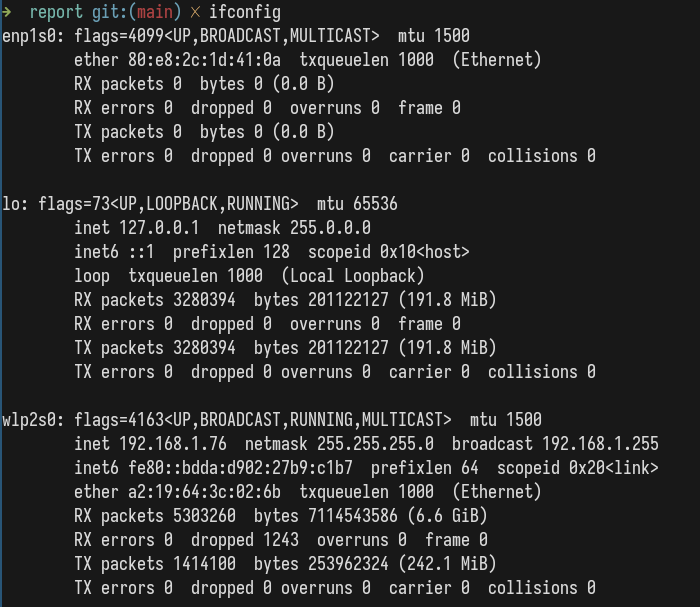
\includegraphics[width=0.8\textwidth]{../images/image01.png}
    \captionof{figure}{Вывод команды ifconfig.}
\end{frame}

\begin{frame}[containsverbatim]
\frametitle{Анализ кадров канального уровня в Wireshark}
    \begin{minted}{bash}
sudo dnf install wireshark
sudo -i
groupadd wireshark
gpasswd -a dastarikov wireshark
chgrp wireshark /usr/bin/dumpcap
chmod 750 /usr/bin/dumpcap
setcap cap_net_raw,cap_net_admin=eip /usr/bin/dumpcap
    \end{minted}
\end{frame}

\begin{frame}
\frametitle{Анализ кадров канального уровня в Wireshark}
    \centering
    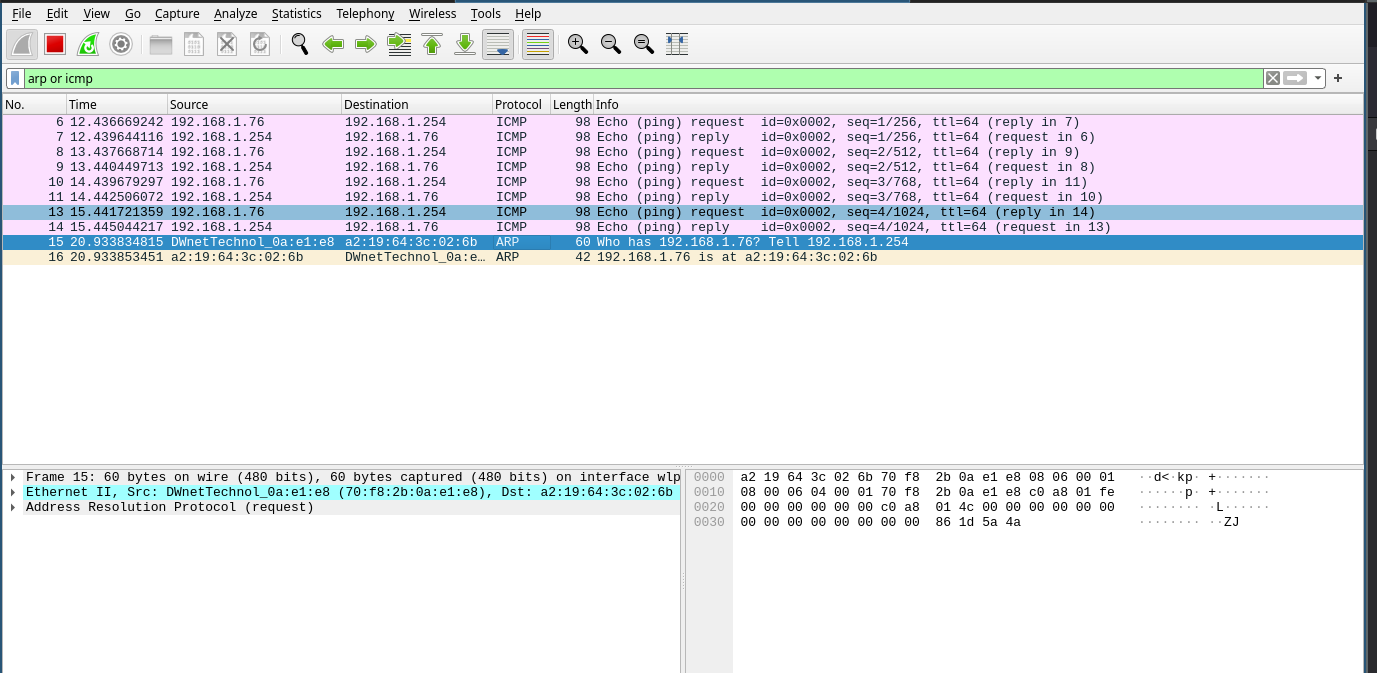
\includegraphics[width=\textwidth]{../images/image10.png}
    \captionof{figure}{Интерфейс Wireshark.}
\end{frame}

\begin{frame}
\frametitle{Анализ кадров канального уровня в Wireshark}
    \centering
    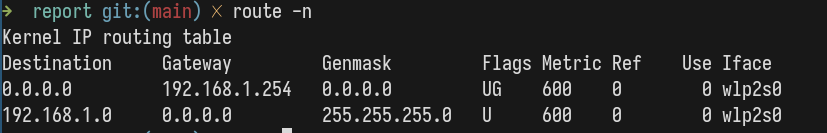
\includegraphics[width=\textwidth]{../images/image07.png}
    \captionof{figure}{Определение IP-адреса шлюза.}
\end{frame}

\begin{frame}
\frametitle{Анализ кадров канального уровня в Wireshark}
    \centering
    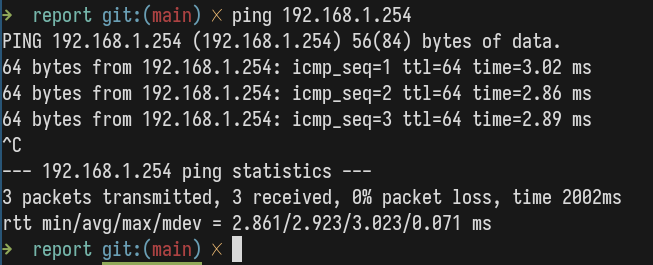
\includegraphics[width=\textwidth]{../images/image08.png}
    \captionof{figure}{Пингование шлюза.}
\end{frame}

\begin{frame}
\frametitle{Анализ кадров канального уровня в Wireshark}
    \centering
    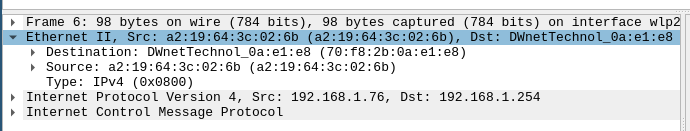
\includegraphics[width=\textwidth]{../images/image11.png}
    \captionof{figure}{Информация об эхо-запросе.}
\end{frame}

\begin{frame}
\frametitle{Анализ кадров канального уровня в Wireshark}
    \centering
    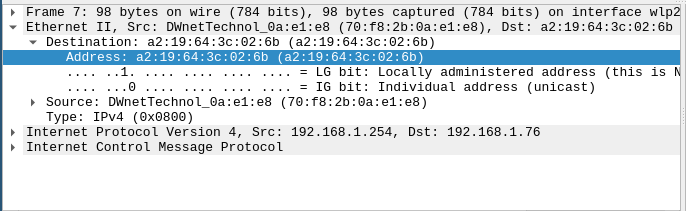
\includegraphics[width=\textwidth]{../images/image12.png}
    \captionof{figure}{Информация об эхо-ответе.}
\end{frame}

\begin{frame}
\frametitle{Анализ кадров канального уровня в Wireshark}
    \centering
    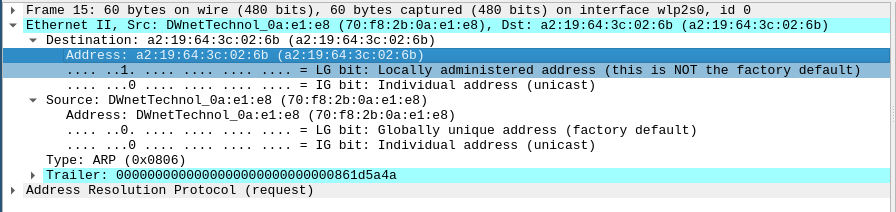
\includegraphics[width=\textwidth]{../images/image13.png}
    \captionof{figure}{Информация кадра протокола ARP.}
\end{frame}

\begin{frame}
\frametitle{Анализ кадров канального уровня в Wireshark}
    \centering
    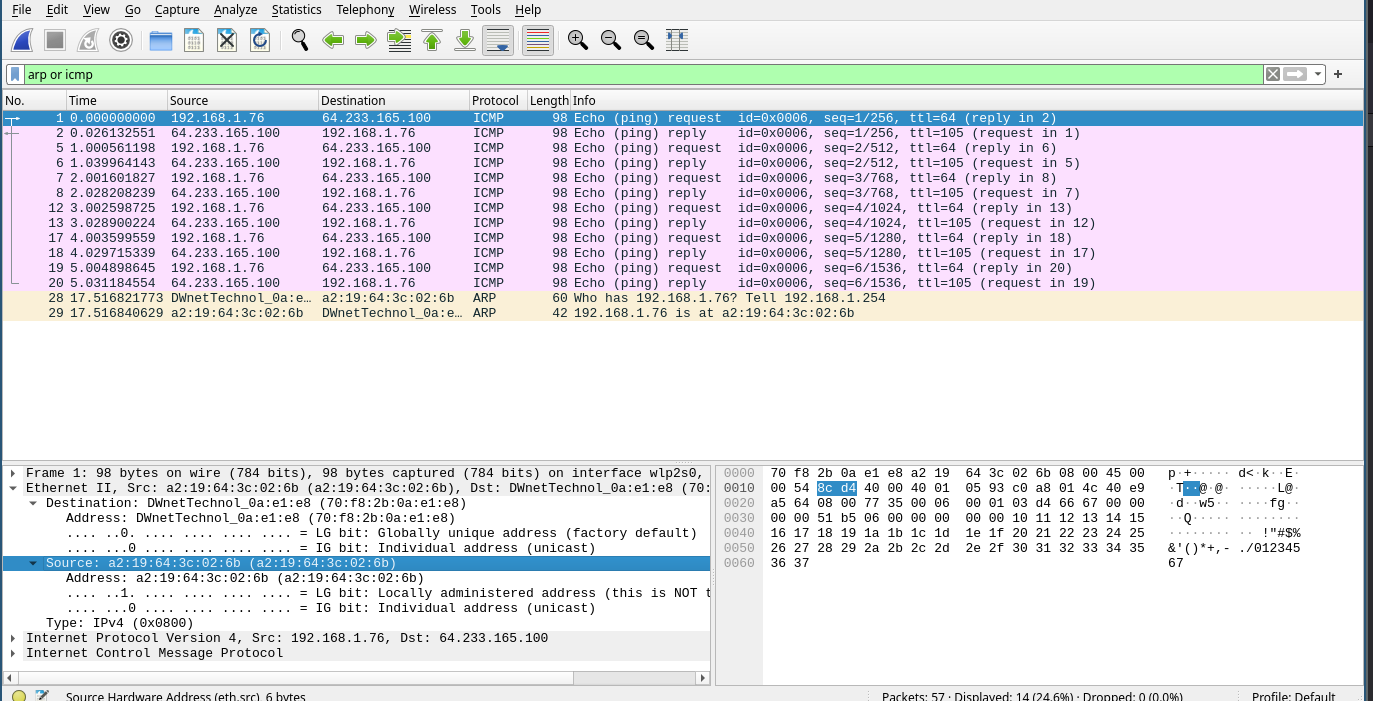
\includegraphics[width=\textwidth]{../images/image15.png}
    \captionof{figure}{Изучение трафика между устройством и google.com.}
\end{frame}

\begin{frame}
\frametitle{Анализ кадров канального уровня в Wireshark}
    \centering
    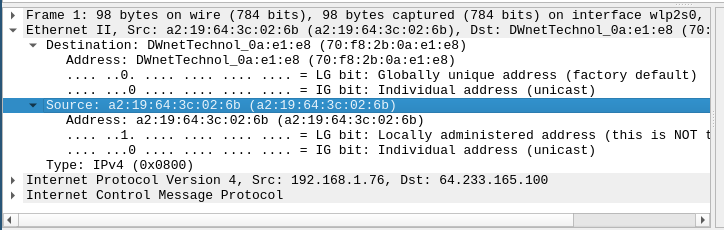
\includegraphics[width=\textwidth]{../images/image16.png}
    \captionof{figure}{Эхо-запрос к google.com}
\end{frame}

\begin{frame}
\frametitle{Анализ кадров канального уровня в Wireshark}
    \centering
    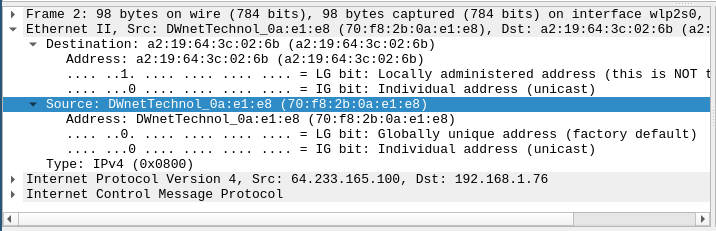
\includegraphics[width=\textwidth]{../images/image17.png}
    \captionof{figure}{Эхо-ответ от google.com}
\end{frame}

\begin{frame}
\frametitle{Анализ протоколов транспортного уровня в Wireshark}
    \centering
    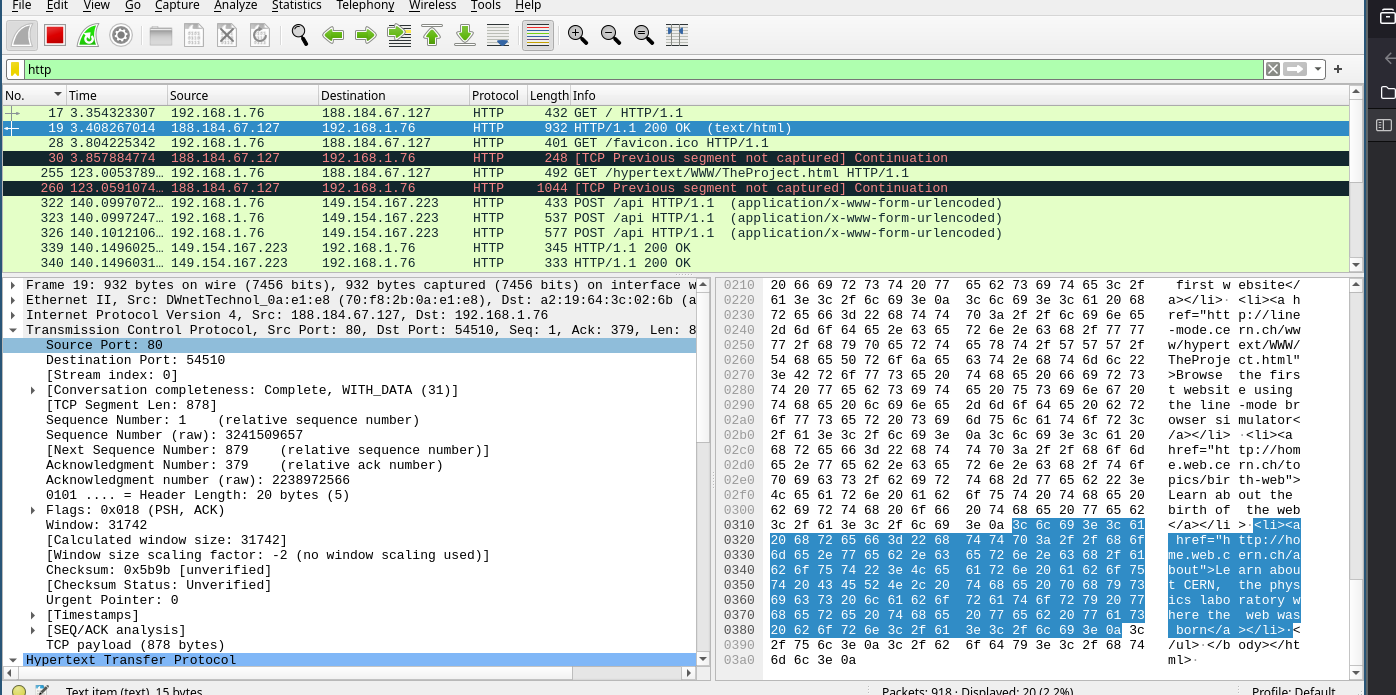
\includegraphics[width=\textwidth]{../images/image18.png}
    \captionof{figure}{Фильтрование трафика по протоколу HTTP.}
\end{frame}

\begin{frame}
\frametitle{Анализ протоколов транспортного уровня в Wireshark}
    \centering
    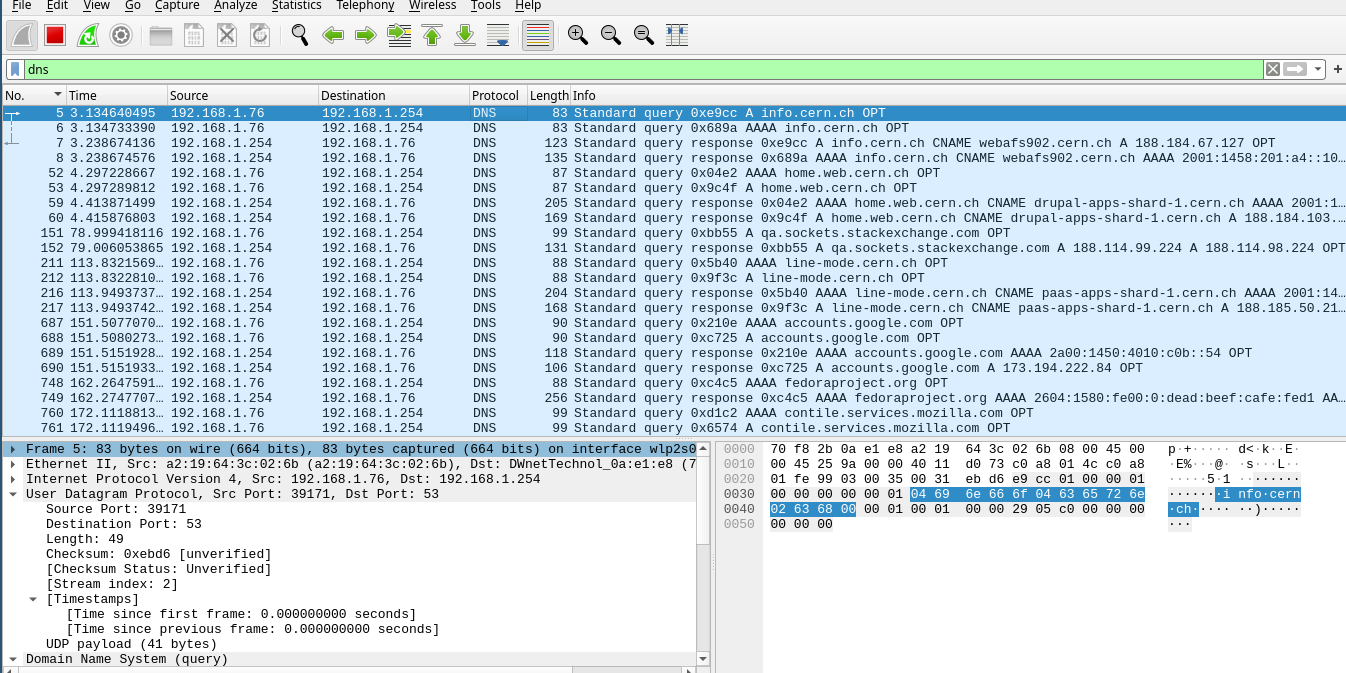
\includegraphics[width=\textwidth]{../images/image19.png}
    \captionof{figure}{Фильтрование трафика по протоколу UDP.}
\end{frame}

\begin{frame}
\frametitle{Анализ протоколов транспортного уровня в Wireshark}
    \centering
    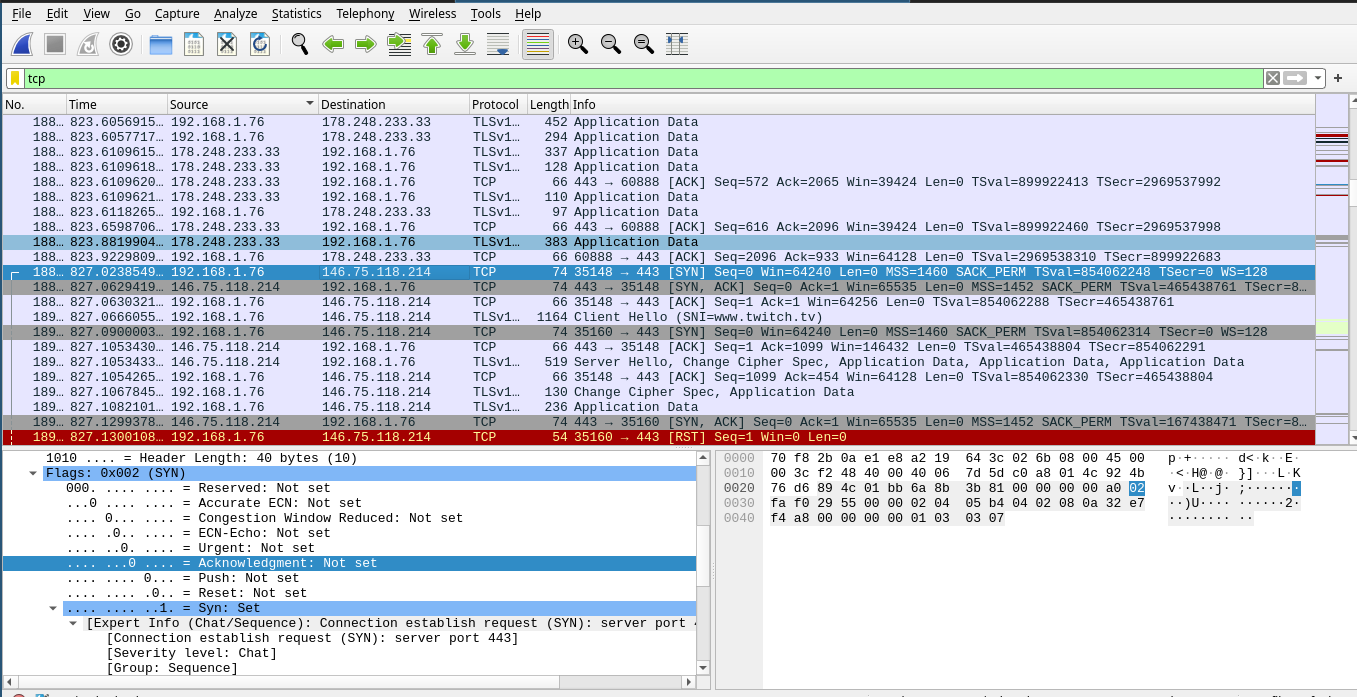
\includegraphics[width=\textwidth]{../images/image22.png}
    \captionof{figure}{handshake протокола TCP.}
\end{frame}

\begin{frame}
\frametitle{Анализ протоколов транспортного уровня в Wireshark}
    \centering
    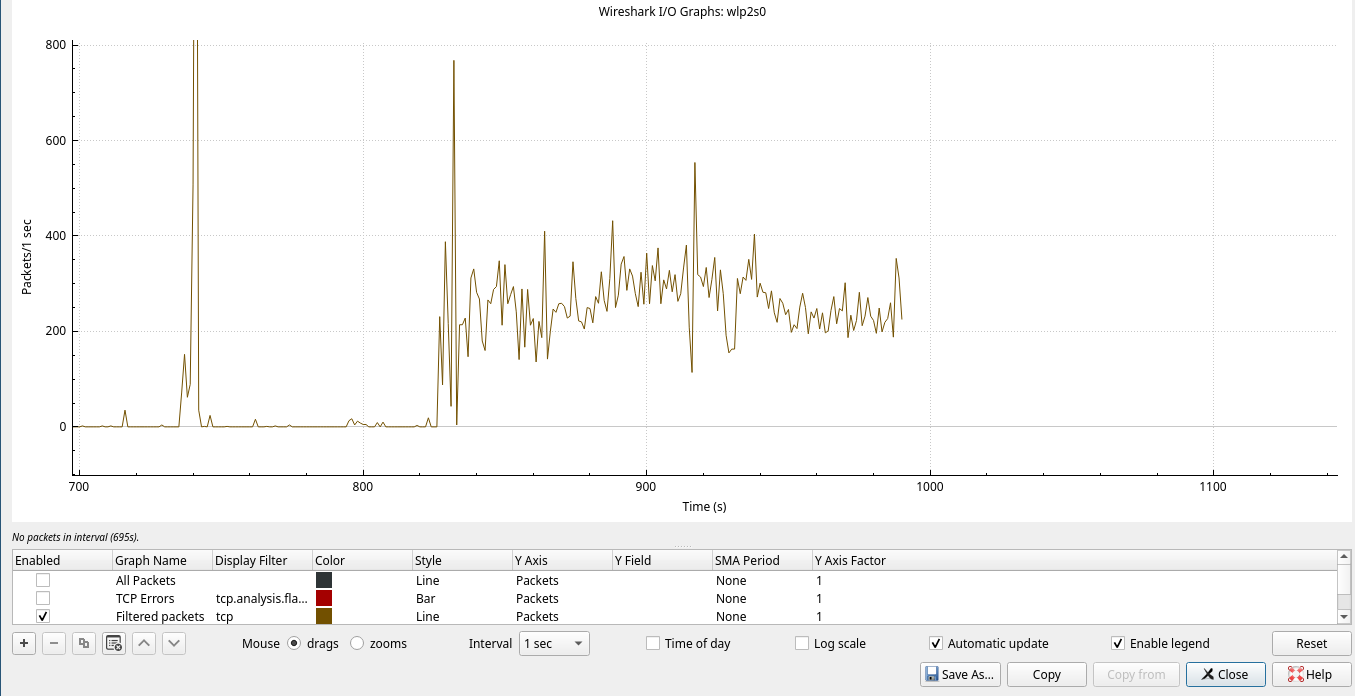
\includegraphics[width=\textwidth]{../images/image23.png}
    \captionof{figure}{График потока TCP пакетов.}
\end{frame}

\begin{frame}
\frametitle{Выводы}
\begin{itemize}
    \item В процессе выполнения лабораторной работы научились работать с программой Wireshark для анализа различных сетевых пакетов на транспортном и прикладном уровнях.
\end{itemize}
\end{frame}
\end{document}
